%%%%%%%%%%%%%%%%%%%%%%%%%%%%%%%%%%%%%%%%%%%%%%%%%%%%%%%%%%%
%% Supporting Information
%%
%% TODO: Free energy corrections to OER intermediates, OER mechanism
%%%%%%%%%%%%%%%%%%%%%%%%%%%%%%%%%%%%%%%%%%%%%%%%%%%%%%%%%%%



% %%%%%%%%%%%%%%%%%%%%%%%%%%%%%%%%%%%%%%%%%%%%%%%%%%%%%%%%%
\subsection{DFT Computational Details}  % %%%%%%%%%%%%%%%%%
% %%%%%%%%%%%%%%%%%%%%%%%%%%%%%%%%%%%%%%%%%%%%%%%%%%%%%%%%%
% Force convergence was 1e-3 for final final bulk opt, and 0.02 for slabs
% Energy SCF convergence was 1e-6 for bulk opt and 1e-5 for slabs
% %%%%%%%%%%%%%%%%%%%%%%%%%%%%%%%%%%%%%%%%%%%%%%%%%%%%%%%%%
% | - DFT Computational Details

% %%%%%%%%%%%%%%%%%%%%%%%%%%%%%%%%%%%%%%%%%%%%%%%%%%%%%%%%%
% | - General intro to shared DFT settings
% Things like the code used
% __|
% %%%%%%%%%%%%%%%%%%%%%%%%%%%%%%%%%%%%%%%%%%%%%%%%%%%%%%%%%
% | - PARAGRAPH BODY
%
Here we describe the density functional theory (DFT) methodology used for both the active learning bulk structure prototype optimization and the OER slab calculations.
%
All calculations were performed using DFT at the generalized gradient approximation (GGA) level of theory as implemented in the Vienna \latin{ab-initio} simulation package (VASP)~\cite{Kresse1995,Kresse1996_0,Kresse1996_1},
and utilizing the PBE exchange-correlation functional~\cite{Perdew1996}.
%
% TODO Cite PAW paper
All calculations were performed with the inclusion of spin-polarization and utilized the projector-augmented wave pseudopotentials (PAW) TEMP.
%
% TODO Cite ASE
Calculations were carried out through the atomic simulation environment (ASE) python interface TEMP.
%
% __|
%%%%%%%%%%%%%%%%%%%%%%%%%%%%%%%%%%%%%%%%%%%%%%%%%%%%%%%%%%%


% %%%%%%%%%%%%%%%%%%%%%%%%%%%%%%%%%%%%%%%%%%%%%%%%%%%%%%%%%
% | - Bulk DFT Specific Settings
%
% __|
% %%%%%%%%%%%%%%%%%%%%%%%%%%%%%%%%%%%%%%%%%%%%%%%%%%%%%%%%%
% | - PARAGRAPH BODY
%
A higher plane-wave cutoff of \SI{600}{\electronvolt} was used for bulk relaxation compared to OER slab calculations (\SI{500}{\electronvolt}).
%
A variable k-point mesh was used such that a k-point density of at least \num{20} k-points per reciprocal space dimension.
%
All bulk systems were run through the following computational recipe to converge the equilibrium structure, with \num{3} distinct phases.
%
structures are only advanced to the next phase when the previous phase completes without error.


\begin{enumerate}
  %
  \item An ISIF \num{7} calculation to optimize only the volume (initial volume of cell may be really off).
  %
  \item Three consecutive ISIF \num{3} relaxations to fully converge the lattice and atomic positions.
  %
  \item A final ISIF \num{2} (fixed unit cell) calculation to relax the atomic coordinates to avoid errors associated with changing the cell volume with a fixed plane-wave cutoff basis.
  %
  This step employs a more stringent SCF convergence criteria of \SI{1e-6}{\electronvolt} and force convergence of \SI{1e-3}{\electronvolt\per\angstrom}
\end{enumerate}
% __|
%%%%%%%%%%%%%%%%%%%%%%%%%%%%%%%%%%%%%%%%%%%%%%%%%%%%%%%%%%%


% %%%%%%%%%%%%%%%%%%%%%%%%%%%%%%%%%%%%%%%%%%%%%%%%%%%%%%%%%
% | - OER Specific Settings
%
% __|
% %%%%%%%%%%%%%%%%%%%%%%%%%%%%%%%%%%%%%%%%%%%%%%%%%%%%%%%%%
% | - PARAGRAPH BODY
%
A 4x4x1 k-point mesh with $\Gamma$-centered Monkshort-packing~\cite{Monkhorst1976} was used for all OER slabs.
%
The plane-wave energy cutoff was \SI{500}{\electronvolt}.
%
% COMBAK Figure out how much spacing was used for all slabs
All slab calculations maintained a vacuum spacing in between TEMP and \SI{15}{\angstrom}.
%
Dipole corrections were imposed on all non-symmetric slabs to counteract spurious dipole interactions between the periodic cells.~\cite{Neugebauer1992}
%
Roughly \num{3/4} of the bottom layers were kept fixed to simulate the bulk crystal while the surface atoms were allowed to fully relax.
%
All structures were relaxed with utilizing the conjugate gradient algorithm as implemented in VASP (IBRION\num{=2}).
%
The simulation stop criteria used was that all atoms must satisfy a maximum force threshold of \SI{0.02}{\electronvolt\per\angstrom}.
% __|
%%%%%%%%%%%%%%%%%%%%%%%%%%%%%%%%%%%%%%%%%%%%%%%%%%%%%%%%%%%

% __|


% %%%%%%%%%%%%%%%%%%%%%%%%%%%%%%%%%%%%%%%%%%%%%%%%%%%%%%%%%
\subsection{Generation of Structural Candidates}  % %%%%%%%
% %%%%%%%%%%%%%%%%%%%%%%%%%%%%%%%%%%%%%%%%%%%%%%%%%%%%%%%%%
%
% %%%%%%%%%%%%%%%%%%%%%%%%%%%%%%%%%%%%%%%%%%%%%%%%%%%%%%%%%
% | - Generation of Structural Candidates

% %%%%%%%%%%%%%%%%%%%%%%%%%%%%%%%%%%%%%%%%%%%%%%%%%%%%%%%%%
% | - Candidate Generation Intro
% Basic intro into candidate generation
% High-level overview again
%   * Data mining OQMD MP fro AB2/3 entries
%   * Reduce data set by eliminating structurally redundant systems
%     * This is done with Ankit's scheme
% __|
% %%%%%%%%%%%%%%%%%%%%%%%%%%%%%%%%%%%%%%%%%%%%%%%%%%%%%%%%%
% | - PARAGRAPH BODY
%
Here we describe the methodology to construct the set of structural candidates in more detail.
%
The first step of the procedure is to mine materials databases for entries with the desired non-element specific stoichiometry (\latin{i.e.} \ABtwo and \ABthree).
%
Since many of the entries in these databases are structurally redundant,
we used a structure classification scheme to reduce the data set to a structurally unique set.
%
Once this is accomplished, the elements of interest were then substituted into the database structures,
which at this point had their original elemental composition from their database.
%
Finally, the structures are isotropically expanded or contracted to accommodate the difference between the atomic radii of the original elements in the structure and the user defined elements.
%
This procedure of ``pre-optimization'' is an important because it generates reasonable initial geometries which would otherwise produce poor fingerprint representations and lead to a large degree of structural shift during the course of DFT optimization.
% __|
%%%%%%%%%%%%%%%%%%%%%%%%%%%%%%%%%%%%%%%%%%%%%%%%%%%%%%%%%%%


% %%%%%%%%%%%%%%%%%%%%%%%%%%%%%%%%%%%%%%%%%%%%%%%%%%%%%%%%%
% | - TEMP
% Data-mining OQMD and MP
% __|
% %%%%%%%%%%%%%%%%%%%%%%%%%%%%%%%%%%%%%%%%%%%%%%%%%%%%%%%%%
% | - PARAGRAPH BODY
%Herein, we take advantage of the structural diversity already present in materials databases to construct our candidates.
%
We utilized two materials databases, the Open Quantum Materials (OQMD) and the Materials Project (MP) databases because of their large and diverse datasets of crystalline inorganic materials.
%
% TODO Approx. when did Ankit parse these databases
At the time that we originally mined these databases (2018), there were \num{61471} inorganic compounds in the MP database and \num{435583} entries in the OQMD database.
%
We note that the databases have expanded the number of entries considerably since we originally parsed them,
although the number of unique crystal polymorphs is not expected to have increase significantly.
% __|
%%%%%%%%%%%%%%%%%%%%%%%%%%%%%%%%%%%%%%%%%%%%%%%%%%%%%%%%%%%


% %%%%%%%%%%%%%%%%%%%%%%%%%%%%%%%%%%%%%%%%%%%%%%%%%%%%%%%%%
% | - Ankit's paragraph on details on structural classification scheme
%
% __|
% %%%%%%%%%%%%%%%%%%%%%%%%%%%%%%%%%%%%%%%%%%%%%%%%%%%%%%%%%
% | - PARAGRAPH BODY
%
The structural classification scheme of Jain \latin{et al.}~\cite{Jain2018} was used assign the crystal prototype,
consisting of standardized space group and Wyckoff positions,
as well as the element-nonspecific stoichiometry of each structure (\num{497054} in total).
%
This prototype designation can serve as a structural fingerprint and has successfully been applied towards the prediction of formation energies of inorganic compounds \cite{Jain2018}.
%
We identified unique structure types by grouping materials according to participating Wyckoff sites.
%
The Wyckoff sites of crystallographic space groups are a collection of fractional coordinates within the unit cell where atoms are allowed to sit in order to satisfy the symmetry of the underlying space group.
%
The 'standard' setting of materials unit cell are identified and atomic positions are mapped to Wyckoff sites using the openly available, crystal symmetry library Spglib~\cite{spglib}.
%
The structures belonging to same crystallographic space group and having the same participating Wyckoff sites have identical crystal symmetry and are grouped together.
%
These groups are referred to as structure-type in this work.
%
Note that the reported participating Wyckoff sites by Spglib are sometimes different for the same crystal due to crystal translation/rotation.
%
We mapped all such related Wyckoff sites to the same structure-type by looping through all allowed crystal symmetry operations of the crystal.
%
Further mathematical details of these operations are available in TEMP.
% ; Ref []
% __|
%%%%%%%%%%%%%%%%%%%%%%%%%%%%%%%%%%%%%%%%%%%%%%%%%%%%%%%%%%%


% %%%%%%%%%%%%%%%%%%%%%%%%%%%%%%%%%%%%%%%%%%%%%%%%%%%%%%%%%
% | - TEMP
%
% __|
% %%%%%%%%%%%%%%%%%%%%%%%%%%%%%%%%%%%%%%%%%%%%%%%%%%%%%%%%%
% | - PARAGRAPH BODY
%
% COMBAK Revise if Ankit's scheme becomes it's own section
% If it's not ready now, let's not include it.
%See section TEMP for more details on the symmetry based structural classification scheme.
%
Once classified, we selected all entries with the desired stoichiometry of \ABtwo and \ABthree,
for which MP has \num{2424} and \num{2341} \ABtwo and \ABthree entries, respectively,
and OQMD has \num{4736} and \num{28883} \ABtwo and \ABthree entries, respectively.
%
The reason that there are considerably more \ABthree compounds in OQMD is due to the extensive compositional permutation of binary alloys in a cubic \ABthree structure.
%
Within each stoichiometry, the structural classification was used to eliminate structurally redundant systems,
\latin{i.e.} systems that share their stoichiometry, space group, and Wyckoff positions.
%
This process reduces the data set to \num{620} and \num{219} unique structures of \ABtwo and \ABthree for MP and \num{397} and \num{194} structurally unique \ABtwo and \ABthree OQMD entries.
%
Combining the MP and OQMD data sets ultimately results in a dataset of \num{688} \ABtwo and \num{254} \ABthree structurally unique candidates.
% __|
%%%%%%%%%%%%%%%%%%%%%%%%%%%%%%%%%%%%%%%%%%%%%%%%%%%%%%%%%%%


% =========================================================
% TABLE ===================================================
% =========================================================
% | - Table | OQMD MP Structures
\begin{table}[!htb]

  \caption{\label{table:database_structures}
    %
    (a) Number of entries in the OQMD and MP materials databases for the \ABtwo and \ABthree stoichiometries.
    %
    (b) Final number of unique structural candidates for \ABtwo and \ABthree.
    }
  %
  % | - Subtable a
  \begin{subtable}{.5\linewidth}
  \centering
  \caption{}
  %
   %
    %
    \begin{tabular}{cccc}
    \textbf{}         & \textbf{}        & \multicolumn{2}{c}{\textbf{Entries}} \\
    \textbf{Database} & \textbf{Stoich.} & \textbf{Total}   & \textbf{Unique}   \\
    OQMD              &                  & 435,583          &                   \\
                      & \ABtwo           & 4,736            & 397               \\
                      & \ABthree         & 28,883           & 194               \\
    \hline
    MP                &                  & 61,471           &                   \\
                      & \ABtwo           & 2,424            & 620               \\
                      & \ABthree         & 2,341            & 219
    \end{tabular}
    %
   %
  %
  \end{subtable}
  % __|
  %
  %
  \newline
  \vspace*{0.8 cm}
  \newline
  %
  %
  % | - Subtable b
  \begin{subtable}{.5\linewidth}
  \centering
  \caption{}
  %
   %
    %
    \begin{tabular}{cc}
    \multicolumn{2}{c}{\textbf{Final Candidate Set}} \\
    \textbf{Stoich.}   & \textbf{Unique Structures}  \\
    \ABtwo             & 697                         \\
    \ABthree           & 259
    \end{tabular}
    %
   %
  %
  \end{subtable}
  % __|
  %
\end{table}
% __| =====================================================
% =========================================================

% __|


% %%%%%%%%%%%%%%%%%%%%%%%%%%%%%%%%%%%%%%%%%%%%%%%%%%%%%%%%%
\subsection{Structure Featurization and Feature Engineering}
% %%%%%%%%%%%%%%%%%%%%%%%%%%%%%%%%%%%%%%%%%%%%%%%%%%%%%%%%%
%
% %%%%%%%%%%%%%%%%%%%%%%%%%%%%%%%%%%%%%%%%%%%%%%%%%%%%%%%%%
% | - Structure Featurization and Feature Engineering

% %%%%%%%%%%%%%%%%%%%%%%%%%%%%%%%%%%%%%%%%%%%%%%%%%%%%%%%%%
% | - Voronoi tesselation and feature reduction
%
% __|
% %%%%%%%%%%%%%%%%%%%%%%%%%%%%%%%%%%%%%%%%%%%%%%%%%%%%%%%%%
% | - PARAGRAPH BODY
The bulk crystal structures studied here,
both the pre-optimized structural candidates and the post-DFT optimized systems,
were converted into numerical fingerprint vectors via the Voronoi tessellation method developed by Ward et al.~\cite{Ward2017}
%
The method produces a \num{271} length fingerprint vector where the \num{271} features encode both for chemical and structural information by way of convoluting atomic properties with Voronoi neighbors.
%
Since we are operating within the fixed composition of \IrOtwo and \IrOthree stoichiometries many of the \num{271} features become redundant (no variance) and thus we were able to immediately reduce the dimensionality of our feature space to \num{101}.
% __|
%%%%%%%%%%%%%%%%%%%%%%%%%%%%%%%%%%%%%%%%%%%%%%%%%%%%%%%%%%%


% %%%%%%%%%%%%%%%%%%%%%%%%%%%%%%%%%%%%%%%%%%%%%%%%%%%%%%%%%
% | - Feature processing and standardization
%
% __|
% %%%%%%%%%%%%%%%%%%%%%%%%%%%%%%%%%%%%%%%%%%%%%%%%%%%%%%%%%
% | - PARAGRAPH BODY
With the number of features reduced, it is then necessary to further process the raw numerical fingerprints to make them amenable for regression and fitting.
%
This included removing highly skewed data points, removing 0-variance features, and normalizing each feature by centering about the mean (mean of 0) and dividing by the features standard deviation (standard deviation of 0).
%
We expect that most of the remaining features are not linearly independent so we next chose to employ an additional feature reduction step by performing a principle-component analysis (PCA).
%
This allowed us to reduce the number of features to \num{10} while still capturing TEMP of the total variance and minimizing the cross-validated prediction MAE (Figure \ref{fig:cv_anal}).
%
This step is also crucial in reducing the computational expense of running the Gaussian Process training procedure.
% __|
%%%%%%%%%%%%%%%%%%%%%%%%%%%%%%%%%%%%%%%%%%%%%%%%%%%%%%%%%%%

% __|


% =========================================================
% FIGURE ==================================================
% | - Figure | Cross-validation analysis ******************
\begin{figure*}[!htb]
\centering
\makebox[\textwidth][c]{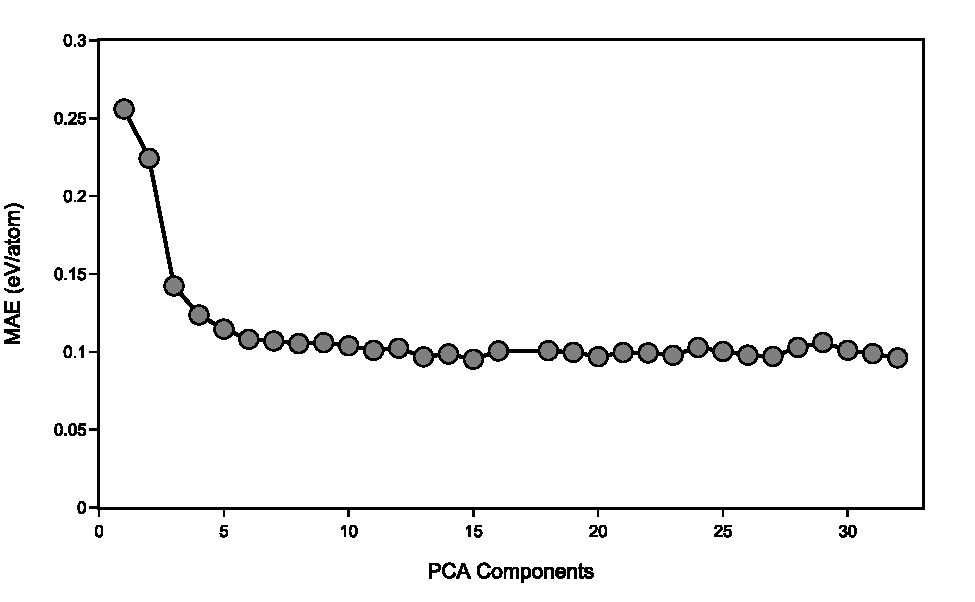
\includegraphics
{02_figures/SI_figures/00_mae_pca_plot__v0.pdf}}
\caption{\label{fig:cv_anal}
20-fold cross validation mean absolute error (MAE) as a function of the number of PCA components used for the GP-regression for \IrOthree.
%
Only post-relaxation fingerprints were used for both training and testing to avoid issues with structural drift.
%
All structural duplicates in the post-relaxation dataset were removed.
}
\end{figure*}
% __|
% =========================================================


% %%%%%%%%%%%%%%%%%%%%%%%%%%%%%%%%%%%%%%%%%%%%%%%%%%%%%%%%%
\subsection{Gaussian Process Regression and Kernel Selection}  % %%%%%%%%%
% %%%%%%%%%%%%%%%%%%%%%%%%%%%%%%%%%%%%%%%%%%%%%%%%%%%%%%%%%
% Relevant details about the ML Gaussian process here
%
% %%%%%%%%%%%%%%%%%%%%%%%%%%%%%%%%%%%%%%%%%%%%%%%%%%%%%%%%%
% | - Gaussian Process Regression and Kernel Selection

% %%%%%%%%%%%%%%%%%%%%%%%%%%%%%%%%%%%%%%%%%%%%%%%%%%%%%%%%%
% | - TEMP
%
% __|
% %%%%%%%%%%%%%%%%%%%%%%%%%%%%%%%%%%%%%%%%%%%%%%%%%%%%%%%%%
% | - PARAGRAPH BODY
%
Gaussian process machine learning regression models were picked due to their highly flexible fits and high performance in situations with small data sets.
%
We utilized the Gaussian Process regression module as implemented in CatLearn.\cite{hansen2019atomistic,CatLearn_Repo}
%
The Gaussian Process recipe we developed utilized two isotropic Gaussian kernels which differ only in the values of the initial length scale parameter ($l$) and scaling parameter ($s$).
%
Here, isotropic refers to keeping the dimensionality of the kernel equal to one instead of an anisotropic kernel which was found to be difficult to optimize.
%
The first GP kernel was constructed with a length scale parameter of \num{1} ($l_1$) and a scaling factor of 5 ($s_1$),
while for the second kernel the length scale and scaling factor were reduced by a factor of ten ($l_2$ and $s_2$).
%
This was done with the aim of producing a model that is responsive to both long- and short-range features in the input space.
%
Additionally, a regularization parameter ($\lambda$) which helps avoid over-fitting was set to an initial value of \num{0.025}.
%
% TODO Double check that I said it correctly, might be minimizing the LML
It should be stressed that these hyper-parameter values are only initial seed values, and that they will be optimized during every round of model training,
which occurs once per active learning loop,
and is done by maximizing the log marginal likelihood of the model and training data.

\begin{equation}
    k(x,x') =
    s_1 exp \Bigl ( \frac{-|x-x'|^2}{2l_1^2}\Bigr) +
    s_2 exp\Bigl (\frac{-|x-x'|^2}{2l_2^2}\Bigr) +
    \lambda \delta_{x,x'}
\end{equation}
% __|
%%%%%%%%%%%%%%%%%%%%%%%%%%%%%%%%%%%%%%%%%%%%%%%%%%%%%%%%%%%

% __|




% %%%%%%%%%%%%%%%%%%%%%%%%%%%%%%%%%%%%%%%%%%%%%%%%%%%%%%%%%
% %%%%%%%%%%%%%%%%%%%%%%%%%%%%%%%%%%%%%%%%%%%%%%%%%%%%%%%%%
% %%%%%%%%%%%%%%%%%%%%%%%%%%%%%%%%%%%%%%%%%%%%%%%%%%%%%%%%%
% %%%%%%%%%%%%%%%%%%%%%%%%%%%%%%%%%%%%%%%%%%%%%%%%%%%%%%%%%
% %%%%%%%%%%%%%%%%%%%%%%%%%%%%%%%%%%%%%%%%%%%%%%%%%%%%%%%%%
% %%%%%%%%%%%%%%%%%%%%%%%%%%%%%%%%%%%%%%%%%%%%%%%%%%%%%%%%%
% %%%%%%%%%%%%%%%%%%%%%%%%%%%%%%%%%%%%%%%%%%%%%%%%%%%%%%%%%
% %%%%%%%%%%%%%%%%%%%%%%%%%%%%%%%%%%%%%%%%%%%%%%%%%%%%%%%%%




% %%%%%%%%%%%%%%%%%%%%%%%%%%%%%%%%%%%%%%%%%%%%%%%%%%%%%%%%%
\subsection{Active Learning Results For \IrOtwo} %
% %%%%%%%%%%%%%%%%%%%%%%%%%%%%%%%%%%%%%%%%%%%%%%%%%%%%%%%%%
% Here are the analogous IrO2 results that were presented for IrO3 in the main text
% %%%%%%%%%%%%%%%%%%%%%%%%%%%%%%%%%%%%%%%%%%%%%%%%%%%%%%%%%
% | - Active Learning Results For \IrOtwo

% %%%%%%%%%%%%%%%%%%%%%%%%%%%%%%%%%%%%%%%%%%%%%%%%%%%%%%%%%
% | - Introduction Paragraph
%
% __|
% %%%%%%%%%%%%%%%%%%%%%%%%%%%%%%%%%%%%%%%%%%%%%%%%%%%%%%%%%
% | - PARAGRAPH BODY
%
Here we outline the results for the AL algorithm applied towards the space of all \IrOtwo candidates.
%
Interactive animations of the active learning loop can be found as supplemental files titled
\texttt{AL\_IrO2\_Animation.html}
and
\texttt{AL\_IrO3\_Animation.html},
which can be opened in any web browser.
% __|
%%%%%%%%%%%%%%%%%%%%%%%%%%%%%%%%%%%%%%%%%%%%%%%%%%%%%%%%%%%


% %%%%%%%%%%%%%%%%%%%%%%%%%%%%%%%%%%%%%%%%%%%%%%%%%%%%%%%%%
% | - IrO2 AL General Results
% TODO Average number of runs to get R-IrO2
% TODO How many gens to obtain x/10
% TODO
% __|
% %%%%%%%%%%%%%%%%%%%%%%%%%%%%%%%%%%%%%%%%%%%%%%%%%%%%%%%%%
% | - PARAGRAPH BODY
%
Figure \ref{fig:iro2_al} shows the results of the active learning framework showcased here applied towards the space of \IrOtwo polymorphs.
%
The structure of Figure \ref{fig:iro2_al} is identical to \ref{fig:iro3_al}, so the reader should refer to the main text for a more elaborate explanation of all the components.
%

In Figure \ref{fig:iro2_al}b six of the seven most stable \IrOtwo polymorphs are displayed.
%
The most stable phase corresponds to \rIrOtwo, the already established globally stable \IrOtwo polymorph,
which illustrates that our methodology can recover known phases readily.
%
Additionally, our AL algorithm recovered other known phases of \IrOtwo, including columbite (\ref{fig:iro2_al}b.vi), pyrite (\ref{fig:iro2_al}b.vii), and anatase (not shown).
% __|
%%%%%%%%%%%%%%%%%%%%%%%%%%%%%%%%%%%%%%%%%%%%%%%%%%%%%%%%%%%


% %%%%%%%%%%%%%%%%%%%%%%%%%%%%%%%%%%%%%%%%%%%%%%%%%%%%%%%%%
% | - IrO2 AL Performance
%
% __|
% %%%%%%%%%%%%%%%%%%%%%%%%%%%%%%%%%%%%%%%%%%%%%%%%%%%%%%%%%
% | - PARAGRAPH BODY
Figure \ref{fig:iro2_al}c presents the discovery rate of the AL loop as a function of DFT bulk optimizations for the case of a GP-LCB acquisition criteria and the baseline random acquisition.
%
The results are qualitatively similar to the case of \IrOthree,
the GP-LCB method readily outperforms the random acquisition.
%
With only \num{200} DFT optimizations (\mytilde40\% of the entire candidate space) the algorithm has discovered \num{9/10}ths of most stable systems,
while the random acquisition requires complete exhaustion of the candidates to find everything.
%
Interestingly the GP-LCB appears to saturate at nine structures, and is unable to find the tenth most stable structure until the candidate space is essentially exhausted.
%
Further investigation reveals that the hold-out structure has a very high predicted formation energy (\DHf),
despite the fact that it's post-DFT structure is the tenth most stable structure in dataset.
%
This result is another manifestation of structural drift between the pre- and post-optimized structures and indicates that the initial candidate structure was initialized in unreasonable coordinates and/or that the structure traversed a long distance through phase space such that the final and initial structures were no longer qualitatively similar.
%
This result highlights the importance of creating reasonable initial candidates.
% __|
%%%%%%%%%%%%%%%%%%%%%%%%%%%%%%%%%%%%%%%%%%%%%%%%%%%%%%%%%%%

% __|


% =========================================================
% FIGURE ==================================================
% =========================================================
% | - Figure | IrO2 Active Learning Results
\begin{figure*}[!htb]
\centering
\makebox[\textwidth][c]{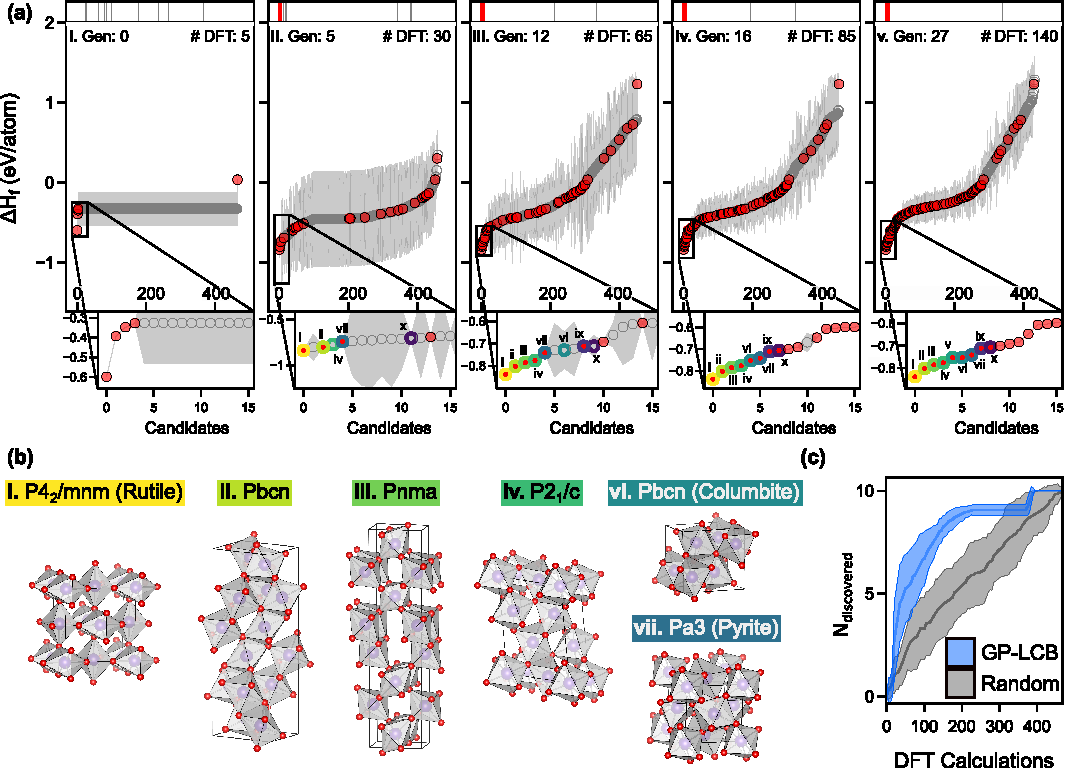
\includegraphics
{02_figures/SI_figures/00_ml_plot_iro2_al__v8__downsampled_1200x1200.pdf}}
\caption{\label{fig:iro2_al}
%
Results for the active learning algorithm applied to the \IrOtwo space.
%
Analogous to Figure \ref{fig:iro3_al}, see Figure \ref{fig:iro3_al} for description of all subplots.
}
\end{figure*}
% __| =====================================================
% =========================================================


% %%%%%%%%%%%%%%%%%%%%%%%%%%%%%%%%%%%%%%%%%%%%%%%%%%%%%%%%%
\subsection{Discovery Rate for All Active Learning Runs} %%
% %%%%%%%%%%%%%%%%%%%%%%%%%%%%%%%%%%%%%%%%%%%%%%%%%%%%%%%%%
% TEMP
% %%%%%%%%%%%%%%%%%%%%%%%%%%%%%%%%%%%%%%%%%%%%%%%%%%%%%%%%%
% | - Discovery rate of all runs of AL algorithms

% %%%%%%%%%%%%%%%%%%%%%%%%%%%%%%%%%%%%%%%%%%%%%%%%%%%%%%%%%
% | - TEMP
%
% __|
% %%%%%%%%%%%%%%%%%%%%%%%%%%%%%%%%%%%%%%%%%%%%%%%%%%%%%%%%%
% | - PARAGRAPH BODY
%
The entire AL algorithm was run a total of \num{100} times for both \IrOtwo and \IrOthree.
%
Each run was independent of the rest, with the only difference being the initial five candidates that were drawn.
%
Figures \ref{fig:iro3_al}c and \ref{fig:iro2_al}c show the results of the average discovery rate of these indpendent runs.
%
Figure \ref{fig:disc_rate} shows the same data, but with each individual run shown.
%
The red traces correspond to the specific runs that were plotted in Figures \ref{fig:iro3_al} and \ref{fig:iro2_al} and were chosen for being representative of the performance of the whole ensemble.
%
It is evident that the GP-LCB method has much less variability in its discovery rate compared to random, which is to say that it can more reliably acquire stable structures when compared to a random walk through the candidates.
% __|
%%%%%%%%%%%%%%%%%%%%%%%%%%%%%%%%%%%%%%%%%%%%%%%%%%%%%%%%%%%

% __|


% =========================================================
% FIGURE ==================================================
% =========================================================
% | - Figure | Discovery rate of all runs of AL algorithms
\begin{figure*}[!htb]
\centering
\makebox[\textwidth][c]{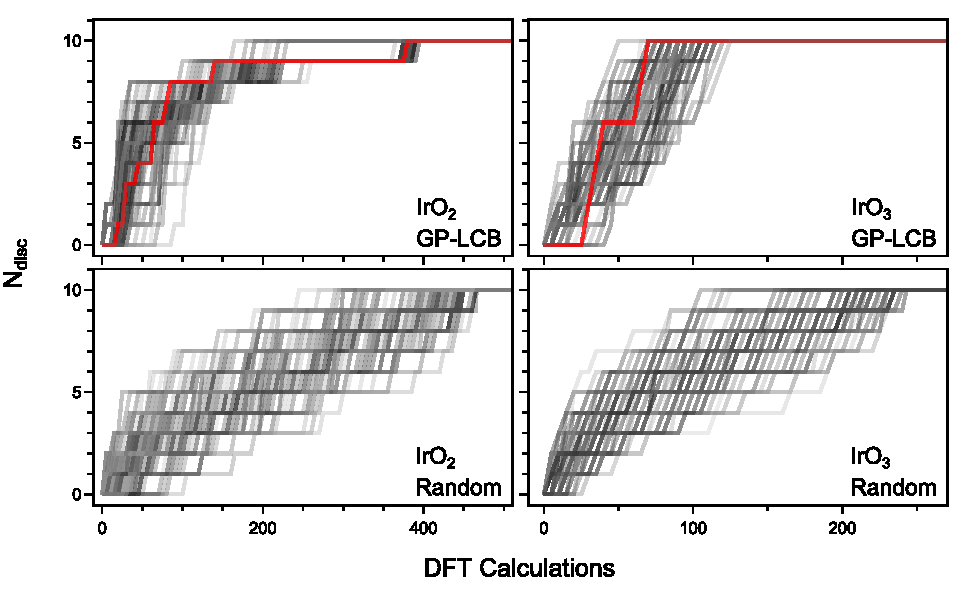
\includegraphics
{02_figures/SI_figures/00_disc_vs_dft__v1.pdf}}
\caption{\label{fig:disc_rate}
%
Quantity of top ten most stable \IrOtwo and \IrOthree polymorphs discovered ($N_{disc}$) as a function of the number of DFT bulk optimizations performed for the GP-LCB acquisition and the baseline random acquisition methods.
%
Red lines indicate the specific runs used for Figures \ref{fig:iro3_al} and Figure \ref{fig:iro2_al}.
}
\end{figure*}
% __| =====================================================
% =========================================================


% % %%%%%%%%%%%%%%%%%%%%%%%%%%%%%%%%%%%%%%%%%%%%%%%%%%%%%%%%%
% \subsection{Structural Coordination Motif Analysis} %
% % %%%%%%%%%%%%%%%%%%%%%%%%%%%%%%%%%%%%%%%%%%%%%%%%%%%%%%%%%
% %
% % %%%%%%%%%%%%%%%%%%%%%%%%%%%%%%%%%%%%%%%%%%%%%%%%%%%%%%%%%
% % | - Structural Coordination Motif Analysis
%
%
% % %%%%%%%%%%%%%%%%%%%%%%%%%%%%%%%%%%%%%%%%%%%%%%%%%%%%%%%%%
% % | - TEMP
% %
% % __|
% % %%%%%%%%%%%%%%%%%%%%%%%%%%%%%%%%%%%%%%%%%%%%%%%%%%%%%%%%%
% % | - PARAGRAPH BODY
% TEMP section about doing the structural motif analysis. Maybe not needed.
% % __|
% %%%%%%%%%%%%%%%%%%%%%%%%%%%%%%%%%%%%%%%%%%%%%%%%%%%%%%%%%%%
%
%
% % __|


% %%%%%%%%%%%%%%%%%%%%%%%%%%%%%%%%%%%%%%%%%%%%%%%%%%%%%%%%%
\subsection{Amorphous Phase Synthesizability Limit and Amorphous Limit}
% %%%%%%%%%%%%%%%%%%%%%%%%%%%%%%%%%%%%%%%%%%%%%%%%%%%%%%%%%
%
% %%%%%%%%%%%%%%%%%%%%%%%%%%%%%%%%%%%%%%%%%%%%%%%%%%%%%%%%%
% | - Amorphous Phase Synthesizability Limit and Amorphous Limit

% %%%%%%%%%%%%%%%%%%%%%%%%%%%%%%%%%%%%%%%%%%%%%%%%%%%%%%%%%
% | - Motivation/Intro to Amorphous Limit
%
% __|
% %%%%%%%%%%%%%%%%%%%%%%%%%%%%%%%%%%%%%%%%%%%%%%%%%%%%%%%%%
% | - PARAGRAPH BODY
To provide a physically motivated energy cut-off for the synthesizability of our polymorphs we employed the procedure from Aykol \latin{et al} for determining the thermodynamic metastability cutoff for crystalline materials based on the amorphous phase limit (amorphous limit).~\cite{Aykol2018}
%
We refer the reader to the full text for a complete explaination of the method,
but briefly, the method uses the formation enthalpy of the most stable amorphous phase as a hard upper limit on the energy of any crystalline polymorph.
%
To obtain the minimum reference energy for the amorphous phase it is necessary to variationally sample low energy amorphous phases,
which was done by sampling low energy configurations from molecular dynamics simulations.
% __|
%%%%%%%%%%%%%%%%%%%%%%%%%%%%%%%%%%%%%%%%%%%%%%%%%%%%%%%%%%%


% %%%%%%%%%%%%%%%%%%%%%%%%%%%%%%%%%%%%%%%%%%%%%%%%%%%%%%%%%
% | - Discussion of Out Data
%
% __|
% %%%%%%%%%%%%%%%%%%%%%%%%%%%%%%%%%%%%%%%%%%%%%%%%%%%%%%%%%
% | - PARAGRAPH BODY
%
This procedure was carried out for both \IrOtwo and \IrOthree (see Table \ref{table:amorph_limit}) and resulted in a amorphous limit (relative to each stoichiometries hull) of
\SI{0.506}{\electronvolt}/atom and \SI{0.307}{\electronvolt}/atom,
respectively.
%
In terms of the formation enthalpy energy scale,
these values convert to
\SI{-0.33}{\electronvolt}/atom and \SI{-0.34}{\electronvolt}/atom
for \IrOtwo and \IrOthree, respectively.
%
It should be stressed, that these values are upper bounds for synthesizability,
and are based on the argument that no ordered crystal structure can exist if its \DHf is less stable than a nearby non-ordered region in phase space.
%
As such, the amorphous limit is stringint boundary on the allowed formation enthalpies of solids but it does not necessarily imply that all structures witin this limit can be physically realized.
% __|
%%%%%%%%%%%%%%%%%%%%%%%%%%%%%%%%%%%%%%%%%%%%%%%%%%%%%%%%%%%

% __|


% =========================================================
% TABLE ===================================================
% =========================================================
% | - Table | Amorphous Limit Data
\begin{table}
\centering
\caption{\label{table:amorph_limit}
%
Density functional thoery computed energetics of sampled amorphous phases for \IrOtwo and \IrOthree as per the procedure of Aykol \latin{et al}~\cite{Aykol2018}.
%
Here we report the raw DFT electronic energy per atom ($E_{DFT}$),
the enthalpy of formation (\DHf),
and the energy above the hull relative to the most stable polymorph of each stoichiometry (\rIrOtwo and \aIrOthree).
%
The most stable amorphous phase for each stoichiometry is bolded.
}
\begin{tabular}{cccccc}
\toprule
       $IrO_{2}$ & \phantom{10.187} &  \phantom{20.395} &        $IrO_{3}$ &  \phantom{10.17} &  \phantom{20.852} \\
       $E_{DFT}$ &   $\Delta H_{f}$ & $\Delta E_{hull}$ &        $E_{DFT}$ &   $\Delta H_{f}$ & $\Delta E_{hull}$ \\
       (eV/atom) &        (eV/atom) &         (eV/atom) &        (eV/atom) &        (eV/atom) &         (eV/atom) \\
\midrule
          -6.493 &           -0.284 &             0.555 &           -6.124 &           -0.305 &             0.346 \\
          -6.523 &           -0.314 &             0.524 &           -6.115 &           -0.296 &             0.355 \\
          -6.464 &           -0.255 &             0.583 &           -6.159 &            -0.34 &             0.311 \\
          -6.503 &           -0.293 &             0.545 &           -6.093 &           -0.274 &             0.377 \\
          -6.528 &           -0.319 &             0.519 &           -6.082 &           -0.263 &             0.388 \\
 \textbf{-6.542} &  \textbf{-0.333} &    \textbf{0.506} &  \textbf{-6.163} &  \textbf{-0.344} &    \textbf{0.307} \\
\bottomrule
\end{tabular}

\end{table}
% __| =====================================================
% =========================================================




% %%%%%%%%%%%%%%%%%%%%%%%%%%%%%%%%%%%%%%%%%%%%%%%%%%%%%%%%%
% %%%%%%%%%%%%%%%%%%%%%%%%%%%%%%%%%%%%%%%%%%%%%%%%%%%%%%%%%
% %%%%%%%%%%%%%%%%%%%%%%%%%%%%%%%%%%%%%%%%%%%%%%%%%%%%%%%%%
% %%%%%%%%%%%%%%%%%%%%%%%%%%%%%%%%%%%%%%%%%%%%%%%%%%%%%%%%%
% %%%%%%%%%%%%%%%%%%%%%%%%%%%%%%%%%%%%%%%%%%%%%%%%%%%%%%%%%
% %%%%%%%%%%%%%%%%%%%%%%%%%%%%%%%%%%%%%%%%%%%%%%%%%%%%%%%%%
% %%%%%%%%%%%%%%%%%%%%%%%%%%%%%%%%%%%%%%%%%%%%%%%%%%%%%%%%%
% %%%%%%%%%%%%%%%%%%%%%%%%%%%%%%%%%%%%%%%%%%%%%%%%%%%%%%%%%























% % %%%%%%%%%%%%%%%%%%%%%%%%%%%%%%%%%%%%%%%%%%%%%%%%%%%%%%%%%
% \subsection{Bulk Pourbaix Diagram}  % %%%%%%%%%%%%%%%%%%%%%
% % %%%%%%%%%%%%%%%%%%%%%%%%%%%%%%%%%%%%%%%%%%%%%%%%%%%%%%%%%
% %
% % %%%%%%%%%%%%%%%%%%%%%%%%%%%%%%%%%%%%%%%%%%%%%%%%%%%%%%%%%
% % | - Bulk Pourbaix Diagram
% %
% The electrochemical bulk Pourbaix diagrams were constructed using the TEMP module from pymatgen.
% % __|


% =========================================================
% FIGURE ==================================================
% =========================================================
% | - Figure | Bulk Pourbaix Diagram
\begin{figure*}[!htb]
\centering
\makebox[\textwidth][c]{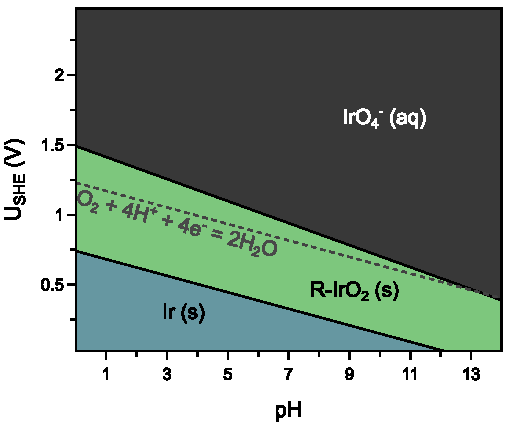
\includegraphics
{02_figures/SI_figures/00_master__bulk-pourbaix__v5.pdf}}
\caption{\label{fig:bulk_pourbaix_wo_alpha}
%
Bulk Pourbaix diagram of the \ce{Ir}-\ce{H2O} system as a function of the applied potential and pH.
%
The diagram was constructed using all of the same species as Figure \ref{fig:bulk_pourbaix} with the exception of the globally stable \IrOthree (\aIrOthree) polymorph.
}
\end{figure*}
% __| =====================================================
% =========================================================


% %%%%%%%%%%%%%%%%%%%%%%%%%%%%%%%%%%%%%%%%%%%%%%%%%%%%%%%%%
\subsection{OER Thermodynamic Methodology}  % %%%%%%%%%%%%%
% %%%%%%%%%%%%%%%%%%%%%%%%%%%%%%%%%%%%%%%%%%%%%%%%%%%%%%%%%
%
% %%%%%%%%%%%%%%%%%%%%%%%%%%%%%%%%%%%%%%%%%%%%%%%%%%%%%%%%%
% | - OER Thermodynamic Methodology
%
Here we will outline the procedure used to carry out OER simulations on the various slabs of \IrOtwo and \IrOthree.
%
The procedure was as follows:
%
Stable stoichiometric terminations were cut from the bulk.
%
% COMBAK
% TODO Add Vesta reference
Stable termination planes were guesstimated via intuition, and the x-ray diffraction pattern tool from Vesta.
%
Next, electrochemical surface coverage was elucidated via a surface Pourbaix analysis.
%
This elucidates the coverage under operating conditions ($>$\num{1.23} \VRHE) for each slab.
%
% COMBAK
Finally we conducted a thermodynamic/limiting potential analysis of the OER mechanistic pathway (Volcano plot, limiting potentials, etc.).
% __|


% %%%%%%%%%%%%%%%%%%%%%%%%%%%%%%%%%%%%%%%%%%%%%%%%%%%%%%%%%
\subsection{Surface Energy Pourbaix Methodology}  % %%%%%%%
% %%%%%%%%%%%%%%%%%%%%%%%%%%%%%%%%%%%%%%%%%%%%%%%%%%%%%%%%%
%
% %%%%%%%%%%%%%%%%%%%%%%%%%%%%%%%%%%%%%%%%%%%%%%%%%%%%%%%%%
% | - Surface Energy Pourbaix Methodology
%
Surface energy Pourbaix plots were constructed by calculating the surface energy of each slab by under standard conditions (\si{\volt}\num{=0} and pH\num{=0}) and then utilizing the computational hydrogen electrode (CHE) to compute the potential dependence of the surfaces.
%
Surface energy calculations were performed for various facets for slabs of increasing thickness.
%
% TODO Insert reference for surface E calcs
The bulk energy was then extracted by fitting the total energy of the slabs against the number of layers as explained in TEMP.
%
This was done to avoid common issues of surface energy divergence associated with using a separate bulk energy calculation.
%
The sensitivity of a given slab to an applied bias is dependent on the composition of the surface,
in particular, the effect of coverage of electrolyte species which can deposit oxygen, hydrogen, and hydroxide species on the surface layers.
%
These additional \ce{O} and \ce{H} atoms are not referenced to the atoms in the slab, but are instead referenced to the computational hydrogen electrode and water-splitting reaction.
%
% TODO Type out equations for surface energy calculation
The equation for is as follows:
% __|


% %%%%%%%%%%%%%%%%%%%%%%%%%%%%%%%%%%%%%%%%%%%%%%%%%%%%%%%%%
\subsection{OER Scaling Relations}  % %%%%%%%%%%%%%%%%%%%%%
% %%%%%%%%%%%%%%%%%%%%%%%%%%%%%%%%%%%%%%%%%%%%%%%%%%%%%%%%%
%
% %%%%%%%%%%%%%%%%%%%%%%%%%%%%%%%%%%%%%%%%%%%%%%%%%%%%%%%%%
% %%%%%%%%%%%%%%%%%%%%%%%%%%%%%%%%%%%%%%%%%%%%%%%%%%%%%%%%%
% | - OER Scaling Relations


% %%%%%%%%%%%%%%%%%%%%%%%%%%%%%%%%%%%%%%%%%%%%%%%%%%%%%%%%%
% | - TEMP
%
% __|
% %%%%%%%%%%%%%%%%%%%%%%%%%%%%%%%%%%%%%%%%%%%%%%%%%%%%%%%%%
% | - PARAGRAPH BODY
%
Figure~\ref{fig:scaling_relations} shows the scaling relations between the adsorption free energies of the OER intermediate species for the studied \IrOx slabs.
%
It can be seen clearly that the data points corresponding to the three \IrOthree polymorphs are roughly \SI{1}{\electronvolt} weaker binding than the \rIrOtwo points.
%
This generally weaker binding of the \IrOthree stoichiometry is responsible for the observed improvement in theoretical activity.
%
The \DGOOH vs.\DGOH relationship is very close to the traditional ``universal scaling relations'', demonstrating that our materials do not break the infamous \DGOOH vs. \DGOH scaling.

% __|
%%%%%%%%%%%%%%%%%%%%%%%%%%%%%%%%%%%%%%%%%%%%%%%%%%%%%%%%%%%


% __|


% =========================================================
% FIGURE ==================================================
% =========================================================
% | - Figure | OER Scaling Relations
\begin{figure*}[!htb]
\centering
\makebox[\textwidth][c]{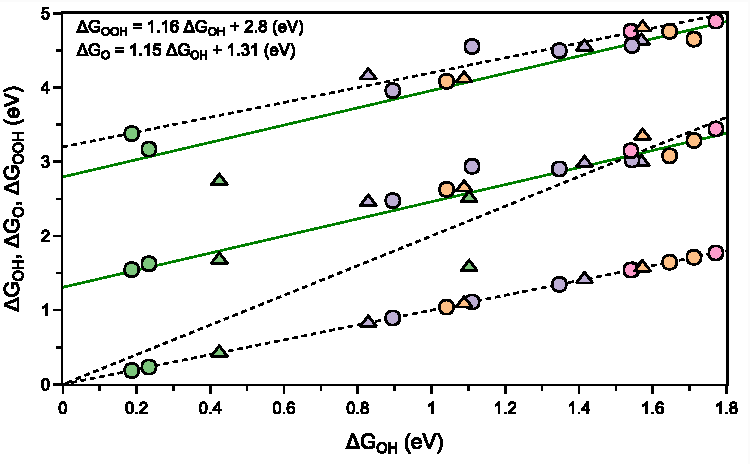
\includegraphics
{02_figures/SI_figures/00_master__oer_scaling__main_v3.pdf}}
\caption{\label{fig:scaling_relations}
%
Relationship between the adsorption free energies of the three key OER intermediates (*OH, *O, *OOH), with \DGOH chosen as the dependent variable.
%
Best fit lines are provided for \DGOOH vs. \DGOH and \DGO vs. \DGOH.
%
Additionally, ``universal scaling relations'' for \DGOOH vs. \DGOH and \DGO vs. \DGOH are shown (black dotted lines) to emphasize our deviation from the traditionally reported scaling fits.
%
The \DGOH line is shown as guide to eye.
% TODO Do I have to redefine the color convention every caption?
}
\end{figure*}
% __| =====================================================
% =========================================================


% %%%%%%%%%%%%%%%%%%%%%%%%%%%%%%%%%%%%%%%%%%%%%%%%%%%%%%%%%
\subsection{Table of OER energetics}  % %%%%%%%%%%%%%%%%%%%
% %%%%%%%%%%%%%%%%%%%%%%%%%%%%%%%%%%%%%%%%%%%%%%%%%%%%%%%%%
%
% %%%%%%%%%%%%%%%%%%%%%%%%%%%%%%%%%%%%%%%%%%%%%%%%%%%%%%%%%
% %%%%%%%%%%%%%%%%%%%%%%%%%%%%%%%%%%%%%%%%%%%%%%%%%%%%%%%%%
% | - Table of OER energetics


% %%%%%%%%%%%%%%%%%%%%%%%%%%%%%%%%%%%%%%%%%%%%%%%%%%%%%%%%%
% | - TEMP
%
% __|
% %%%%%%%%%%%%%%%%%%%%%%%%%%%%%%%%%%%%%%%%%%%%%%%%%%%%%%%%%
% | - PARAGRAPH BODY
%
Table \ref{table:oer_data} contains the adsorbate binding energetics for the intermediates of the OER
oxygen evolution reaction (*O, *OOH, *OH).
% __|
%%%%%%%%%%%%%%%%%%%%%%%%%%%%%%%%%%%%%%%%%%%%%%%%%%%%%%%%%%%


% __|


% =========================================================
% TABLE ===================================================
% =========================================================
% | - Table | OER energetics
\newpage  % request a new page.
\begin{landscape}
\renewcommand{\arraystretch}{1.5} % <--------------
\begin{table}
\resizebox{\linewidth}{!}{%
\centering
\caption{\label{table:oer_data}
%
OER adsorption energies for slabs of \IrOtwo and \IrOthree polymorphs studied here.
%
Included quantities are electronic adsorption energies
($\Delta E_{*O_{x}H_{y}}$),
adsorption free energies
($\Delta G_{*O_{x}H_{y}}$),
as well as the \DGOmOH{} OER descriptor.
%
Coverage indicates the electrochemical coverage of either *O or *OH species.
%
The limiting potential and corresponding overpotential ($\eta$) as well as the rate determining step (RDS) for the OER mechanism are shown.
}
\begin{tabular}{lllcccccccccc}
\toprule
                Bulk Sys. &    Facet &    Coverage & $\Delta E_{*OH}$ & $\Delta E_{*O}$ & $\Delta E_{*OOH}$ & $\Delta G_{*OH}$ & $\Delta G_{*O}$ & $\Delta G_{*OOH}$ & $\Delta G_{*O}-\Delta G_{*OH}$ & Lim. Pot. & $\eta$ &                                                                    RDS \\
                        - &        - &           - &             (eV) &            (eV) &              (eV) &             (eV) &            (eV) &              (eV) &                           (eV) &       (V) &    (V) &                                                                      - \\
\midrule
      $R{\text -}IrO_{2}$ &    (100) &         *OH &            0.130 &           1.634 &             2.362 &            0.424 &           1.678 &             2.738 &                          1.254 &     2.182 &  0.952 &              $*OOH \rightarrow * \phantom{T} \phantom{T} \phantom{T} $ \\
      $R{\text -}IrO_{2}$ &    (100) &          *O &           -0.061 &           1.582 &             2.793 &            0.234 &           1.626 &             3.170 &                          1.392 &     1.750 &  0.520 &              $*OOH \rightarrow * \phantom{T} \phantom{T} \phantom{T} $ \\
      $R{\text -}IrO_{2}$ &    (110) &         *OH &            0.807 &           1.535 &             2.133 &            1.102 &           1.579 &             2.509 &                          0.477 &     2.411 &  1.181 &              $*OOH \rightarrow * \phantom{T} \phantom{T} \phantom{T} $ \\
      $R{\text -}IrO_{2}$ &    (110) &          *O &           -0.108 &           1.503 &             3.004 &            0.187 &           1.547 &             3.380 &                          1.360 &     1.833 &  0.603 &                         $*O \phantom{T} \phantom{T}  \rightarrow *OOH$ \\
 $\alpha{\text -}IrO_{3}$ &    (100) &         *OH &            1.275 &           2.950 &             4.254 &            1.569 &           2.994 &             4.630 &                          1.424 &     1.636 &  0.406 &                         $*O \phantom{T} \phantom{T}  \rightarrow *OOH$ \\
 $\alpha{\text -}IrO_{3}$ &    (100) &          *O &            1.249 &           2.980 &             4.191 &            1.544 &           3.024 &             4.567 &                          1.480 &     1.544 &  0.314 &  $* \phantom{T} \phantom{T} \phantom{T}  \rightarrow *OH \phantom{T} $ \\
 $\alpha{\text -}IrO_{3}$ &    (110) &         *OH &            0.534 &           2.414 &             3.786 &            0.828 &           2.458 &             4.163 &                          1.629 &     1.705 &  0.475 &                         $*O \phantom{T} \phantom{T}  \rightarrow *OOH$ \\
 $\alpha{\text -}IrO_{3}$ &    (110) &          *O &            0.600 &           2.432 &             3.582 &            0.895 &           2.476 &             3.959 &                          1.581 &     1.581 &  0.351 &              $*OH \phantom{T} \rightarrow *O \phantom{T} \phantom{T} $ \\
 $\alpha{\text -}IrO_{3}$ &    (111) &          *O &            0.815 &           2.894 &             4.177 &            1.110 &           2.938 &             4.554 &                          1.828 &     1.828 &  0.598 &              $*OH \phantom{T} \rightarrow *O \phantom{T} \phantom{T} $ \\
 $\alpha{\text -}IrO_{3}$ &    (211) &         *OH &            1.120 &           2.937 &             4.173 &            1.415 &           2.981 &             4.549 &                          1.566 &     1.568 &  0.338 &                         $*O \phantom{T} \phantom{T}  \rightarrow *OOH$ \\
 $\alpha{\text -}IrO_{3}$ &    (211) &          *O &            1.052 &           2.860 &             4.122 &            1.347 &           2.904 &             4.499 &                          1.558 &     1.594 &  0.364 &                         $*O \phantom{T} \phantom{T}  \rightarrow *OOH$ \\
  $\beta{\text -}IrO_{3}$ &  (010)-A &          *O &            1.246 &           3.105 &             4.383 &            1.541 &           3.149 &             4.759 &                          1.609 &     1.610 &  0.380 &                         $*O \phantom{T} \phantom{T}  \rightarrow *OOH$ \\
  $\beta{\text -}IrO_{3}$ &  (010)-B &          *O &            1.477 &           3.399 &             4.519 &            1.771 &           3.443 &             4.896 &                          1.672 &     1.771 &  0.541 &  $* \phantom{T} \phantom{T} \phantom{T}  \rightarrow *OH \phantom{T} $ \\
      $R{\text -}IrO_{3}$ &    (100) &         *OH &            1.278 &           3.304 &             4.431 &            1.572 &           3.348 &             4.807 &                          1.776 &     1.776 &  0.546 &              $*OH \phantom{T} \rightarrow *O \phantom{T} \phantom{T} $ \\
      $R{\text -}IrO_{3}$ &    (100) &          *O &            1.351 &           3.036 &             4.381 &            1.646 &           3.080 &             4.758 &                          1.435 &     1.677 &  0.447 &                         $*O \phantom{T} \phantom{T}  \rightarrow *OOH$ \\
      $R{\text -}IrO_{3}$ &    (100) &  *O-partial &            1.417 &           3.243 &             4.275 &            1.712 &           3.287 &             4.652 &                          1.575 &     1.712 &  0.482 &  $* \phantom{T} \phantom{T} \phantom{T}  \rightarrow *OH \phantom{T} $ \\
      $R{\text -}IrO_{3}$ &    (110) &         *OH &            0.794 &           2.607 &             3.744 &            1.088 &           2.651 &             4.121 &                          1.563 &     1.563 &  0.333 &              $*OH \phantom{T} \rightarrow *O \phantom{T} \phantom{T} $ \\
      $R{\text -}IrO_{3}$ &    (110) &          *O &            0.746 &           2.583 &             3.708 &            1.041 &           2.627 &             4.084 &                          1.586 &     1.586 &  0.356 &              $*OH \phantom{T} \rightarrow *O \phantom{T} \phantom{T} $ \\
\bottomrule
\end{tabular}

}
\end{table}

\end{landscape}
% __| =====================================================
% =========================================================



% | - WORK IN PROGRESS

% %%%%%%%%%%%%%%%%%%%%%%%%%%%%%%%%%%%%%%%%%%%%%%%%%%%%%%%%%
% %%%%%%%%%%%%%%%%%%%%%%%%%%%%%%%%%%%%%%%%%%%%%%%%%%%%%%%%%
% %%%%%%%%%%%%%%%%%%%%%%%%%%%%%%%%%%%%%%%%%%%%%%%%%%%%%%%%%
% %%%%%%%%%%%%%%%%%%%%%%%%%%%%%%%%%%%%%%%%%%%%%%%%%%%%%%%%%
% %%%%%%%%%%%%%%%%%%%%%%%%%%%%%%%%%%%%%%%%%%%%%%%%%%%%%%%%%
% %%%%%%%%%%%%%%%%%%%%%%%%%%%%%%%%%%%%%%%%%%%%%%%%%%%%%%%%%
% %%%%%%%%%%%%%%%%%%%%%%%%%%%%%%%%%%%%%%%%%%%%%%%%%%%%%%%%%
% %%%%%%%%%%%%%%%%%%%%%%%%%%%%%%%%%%%%%%%%%%%%%%%%%%%%%%%%%

% % %%%%%%%%%%%%%%%%%%%%%%%%%%%%%%%%%%%%%%%%%%%%%%%%%%%%%%%%%
% \subsection{Bulk Systems}  % %%%%%%%%%%%%%%%%%%%%%%%%%%%%%%
% % %%%%%%%%%%%%%%%%%%%%%%%%%%%%%%%%%%%%%%%%%%%%%%%%%%%%%%%%%
% %
% % %%%%%%%%%%%%%%%%%%%%%%%%%%%%%%%%%%%%%%%%%%%%%%%%%%%%%%%%%
% % %%%%%%%%%%%%%%%%%%%%%%%%%%%%%%%%%%%%%%%%%%%%%%%%%%%%%%%%%
% % | - Bulk Systems
%
%
% % %%%%%%%%%%%%%%%%%%%%%%%%%%%%%%%%%%%%%%%%%%%%%%%%%%%%%%%%%
% % | - TEMP
% %
% % __|
% % %%%%%%%%%%%%%%%%%%%%%%%%%%%%%%%%%%%%%%%%%%%%%%%%%%%%%%%%%
% % | - PARAGRAPH BODY
% % Formation energies of 4 polymorphs
% % __|
% %%%%%%%%%%%%%%%%%%%%%%%%%%%%%%%%%%%%%%%%%%%%%%%%%%%%%%%%%%%
%
%
% % __|

% %%%%%%%%%%%%%%%%%%%%%%%%%%%%%%%%%%%%%%%%%%%%%%%%%%%%%%%%%
% %%%%%%%%%%%%%%%%%%%%%%%%%%%%%%%%%%%%%%%%%%%%%%%%%%%%%%%%%
% %%%%%%%%%%%%%%%%%%%%%%%%%%%%%%%%%%%%%%%%%%%%%%%%%%%%%%%%%
% %%%%%%%%%%%%%%%%%%%%%%%%%%%%%%%%%%%%%%%%%%%%%%%%%%%%%%%%%
% %%%%%%%%%%%%%%%%%%%%%%%%%%%%%%%%%%%%%%%%%%%%%%%%%%%%%%%%%
% %%%%%%%%%%%%%%%%%%%%%%%%%%%%%%%%%%%%%%%%%%%%%%%%%%%%%%%%%
% %%%%%%%%%%%%%%%%%%%%%%%%%%%%%%%%%%%%%%%%%%%%%%%%%%%%%%%%%
% %%%%%%%%%%%%%%%%%%%%%%%%%%%%%%%%%%%%%%%%%%%%%%%%%%%%%%%%%


% __|
